\documentclass[10pt,a4paper,table]{article}
	
	\usepackage{amsmath,amssymb,amsthm,mathtools,amsfonts}
	\usepackage{breqn}
	\usepackage[utf8]{inputenc}
	\usepackage[danish]{babel}
	\usepackage[T1]{fontenc}
	
	%%%%%%%%%%%%%%%%%%%%%%%%%%%%%%%%%%%%%%%%%%%%%%%%%%%%%%%%%%%%%%%%%%%%%%%%%%%%%% Fonts
	
	\usepackage{fontspec}
	\setmainfont{Times New Roman}
	\newfontfamily\garamond[Numbers=OldStyle]{EB Garamond}
	\newfontfamily\plantin[Numbers=OldStyle]{Plantin MT Pro}
	\newfontfamily\wal{Walbaum Com}
	\newfontfamily\klav{Klavika}
	\newfontfamily\klavl{Klavika light}
	\newfontfamily\quotefont[Ligatures=TeX]{Linux Libertine O}
	\newfontfamily\vest{TRY Vesterbro Regular}
	\newfontfamily\vestb{TRY Vesterbro Poster}
	\newfontfamily\overp{Overpass}
	
	%%%%%%%%%%%%%%%%%%%%%%%%%%%%%%%%%%%%%%%%%%%%%%%%%%%%%%%%%%%%%%%%%%%%%%%%%%%%%% Colors
	
	\usepackage{xcolor}
	
	\definecolor{frbblue}{RGB}{47, 88, 109}
	\definecolor{hgred}{RGB}{140, 10, 10}
	\definecolor{frbgreenl}{RGB}{162, 202, 137}
	\definecolor{frbgreen}{RGB}{28, 85, 66}
	\definecolor{frbgrey}{RGB}{243, 245, 242}
	
	%%%%%%%%%%%%%%%%%%%%%%%%%%%%%%%%%%%%%%%%%%%%%%%%%%%%%%%%%%%%%%%%%%%%%%%%%%%%%% Other Graphics
	
	\usepackage{graphicx}
	\graphicspath{{../img/}}
	\usepackage{tikz}
	\usepackage{placeins}
	\usepackage{subcaption}
	
	\usepackage[pdfborder={0 0 0}]{hyperref} %% Ingen firkant rundt om referencer

	\usepackage{multicol}
	\usepackage{cellspace}
		\setlength\cellspacetoplimit{100pt}
		\setlength\cellspacebottomlimit{100pt}
	\usepackage{tabularx}
		\newcolumntype{b}{>{\hsize=\hsize}>{\centering\arraybackslash}X}
	\usepackage{siunitx}
	\usepackage{cellspace}
		\setlength\cellspacetoplimit{4pt}
		\setlength\cellspacebottomlimit{4pt}
	
	\usepackage{enumitem}% better controls with enumerating
	\usepackage{wrapfig}
	\usepackage{caption}
	%\usepackage{dirtytalk}
	%\usepackage{tasks}
	\usepackage{titlesec}

	\setlength{\parskip}{0.5\baselineskip}
	\setlength{\parindent}{0cm}
	\setlist[enumerate]{label=\alph*),left=20pt}
	%\setlist[enumerate]{leftmargin=\parindent}
	%\setlist[enumerate]{nosep}
	
	
	%%%%%%%%%%%%%%%%%%%%%%%%%%%%%%%%%%%%%%%%%%%%%%%%%%%%%%%%%%%%%%%%%%%%%%%%%%%%%% New commands
	
	\newcommand\svar[1]{\newline\textcolor{red}{\textbf{Svar}\\#1}}
	
	\usepackage[h]{esvect}
	\newcommand{\twvect}[2]{\ensuremath{\begin{pmatrix}#1\\#2\end{pmatrix}}}
	
	\newcommand*\quotesize{20}
	\newcommand*{\openquote}
		{\tikz[remember picture,overlay,xshift=-3ex,yshift=-0ex]
			\node (OQ) {\quotefont\fontsize{\quotesize}{\quotesize}\selectfont``};\kern0pt}

	\newcommand*{\closequote}[1]
		{\tikz[remember picture,overlay,xshift=2ex,yshift={#1}]
			\node (CQ) {\quotefont\fontsize{\quotesize}{\quotesize}\selectfont''};}
			
	\newcommand{\qm}[1]{``#1''}
	\newcommand{\iquote}[1]{\begin{quote}\itshape \openquote#1\hfill\closequote{0ex} \end{quote}}
	
	%%%%%%%%%%%%%%%%%%%%%%%%%%%%%%%%%%%%%%%%%%%%%%%%%%%%%%%%%%%%%%%%%%%%%%%%%%%%%% Sections
	\usepackage{chngcntr}
	
	\renewcommand\thesection{\arabic{section}}

	\titleformat{\section}[block] 
  		{\flushright\overp\Large\color{frbgreen}}    % format for whole title
  		{}                           % no separate label (empty)
  		{0pt}                        % spacing between label and title
		{DELPRØVE \thesection}       % prepend "Delprøve <number>"
		[{\color{frbgreenl}\vspace{-1em}\hspace*{-0.165\linewidth}\rule{\dimexpr1.165\linewidth\relax}{0.4pt}\kern1mm}]
	
	\counterwithout{subsection}{section}
	\renewcommand\thesubsection{Opgave \arabic{subsection}}
	\titleformat{\subsection}[leftmargin]{\bfseries}{}{0pt}{\hspace{-5em}\thesubsection}
	
	%%%%%%%%%%%%%%%%%%%%%%%%%%%%%%%%%%%%%%%%%%%%%%%%%%%%%%%%%%%%%%%%%%%%%%%%%%%%%% Header & Footer
	
	\usepackage{bigfoot}
	\DeclareNewFootnote{a}
		\renewcommand{\thefootnotea}{\fnsymbol{footnotea}}
			\newcommand{\footnotes}[1]{\footnotea[2]{#1}} % here you can specify what symbol you want in footnotes
			\MakePerPage{footnotes}
	
		\usepackage{fancyhdr}
	\fancypagestyle{plain}{%
		\setlength{\headheight}{60pt}%
		\setlength{\headsep}{0pt}
		\fancyhf{}% No header/footer
		\renewcommand{\footrulewidth}{0pt}% No footer rule
		\renewcommand\headrule{
			\centerline{\begin{minipage}{1\textwidth}
				\color{frbblue}\hrule width \hsize \kern 1mm \hrule width \hsize height 2pt \vspace{4em}
			\end{minipage}}
		}
		\fancyhead[L]{\hspace{0em}
\includegraphics[height=2.5em]{frbvuc_logo.png}}
		\fancyhead[R]{\overp\color{frbgreen}\footnotesize Forår 2026}
		\fancyhead[C]{\overp\color{frbgreenl}\normalsize \overp Mat C-B\\\Large\color{frbgreen}\vestb Aflevering 10}
		\cfoot{\thepage}
	}
	\pagestyle{fancy}
	\fancyhf{}
	\renewcommand\headrule{
			\centerline{\begin{minipage}{\textwidth}
				\color{frbgreen}\hrule width \hsize \kern 1mm
			\end{minipage}}}
	\lhead{\overp\color{frbgreen}\footnotesize Mat C-B}
	\rhead{\overp\color{frbgreen}\footnotesize Forår 2026}
	\cfoot{\thepage}
	
	%%%%%%%%%%%%%%%%%%%%%%%%%%%%%%%%%%%%%%%%%%%%%%%%%%%%%%%%%%%%%%%%%%%%%%%%%%%%%% Document

\begin{document}
\thispagestyle{plain}

I beviset for løsningsformlen for andengradsligningen $a\cdot x^2+b\cdot x+c=0$ lavede vi en omskrivning af ligningen, hvor vi "færdiggjorde" kvadratet ved hjælp af kvadratsætningerne. Denne omskrivning kaldes en kvadratkomplettering. Denne rene algebraiske øvelse kan virke mærkelig abstrakt; hvor kommer $4a$ f.eks. fra? Ligninger har dog historisk været langt tættere forbundet med geometriske problemer. Hvordan man kan anskue løsning af ligninger som geometri, skal vi se nærmere på i dette projekt.

I 800-tallet skrev den persiske matematiker Al-Khwarizmi om ligninger på en måde, som blev vigtig for algebraens tidlige udvikling. Hans fremstilling var dog ikke symbolsk som den algebra, vi bruger i dag; i stedet blev regneregler og løsninger beskrevet med ord og ofte begrundet geometrisk.

Hvordan man kan begrunde geometrisk kan vi forstå ved at se på et eksempel. Se for eksempel på andengradsudtrykket:
\[
x^2+6x+20.
\]
Her kan første led tolkes som arealet af et kvadrat med siden $x$. Tilsvarende kan andet led tolkes som arealet af et rektangel med siderne $6$ og $x$. Endelig kan det tredje led opfattes som arealet af en uspecificeret figur.

\begin{figure}[h!]
\centering
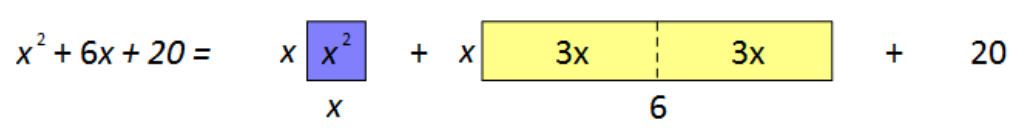
\includegraphics[width=0.8\textwidth]{kvadratkomplettering_1}
\end{figure}

Halveres rektanglet, kan de to dele flyttes rundt, så figuren næsten bliver til et stort kvadrat.

\begin{figure}[h!]
\centering
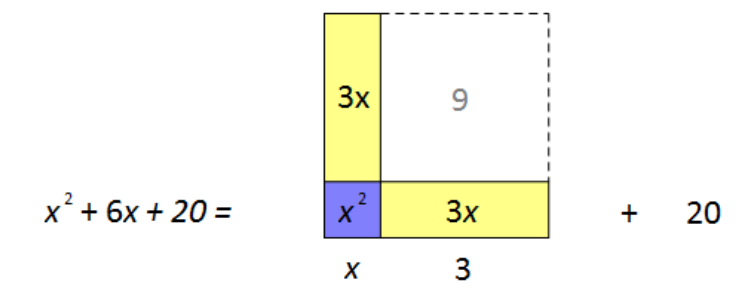
\includegraphics[width=0.8\textwidth]{kvadratkomplettering_2}
\end{figure}

Nu ser vi, at der kun mangler et kvadrat med siden $3$ for at fuldende figuren. Vi l\aa ner derfor arealet $9$ fra konstantleddet og f\aa r omskrevet udtrykket til summen af et stort kvadrat og en ny konstant:

\begin{figure}[h!]
\centering
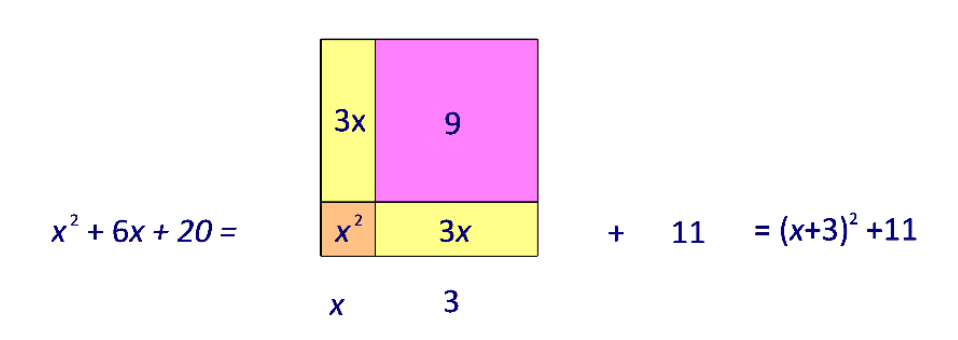
\includegraphics[width=0.8\textwidth]{kvadratkomplettering_3}
\end{figure}

Dermed f\aa r vi
\[
x^2+6x+20=(x+3)^2+11.
\]
Denne visuelle tilgang har spillet en vigtig rolle langt tilbage i matematikkens historie. Først senere blev algebra i stigende grad udviklet som en mere symbolsk og abstrakt disciplin.

\subsection{}
Lad os her prøve at gøre kvadrater helt konkrete. Forestil jer hvert led i følgende udregninger som arealet af en firkant. Kan man udregne det samlede areal som arealet af et enkelt kvadrat i stedet? Illustrer hvert eksempel.
\begin{enumerate}
  \item $x^2+6x+9$
  \item $x^2+2x+1$
  \item $x^2+12x+36$
  \item $x^2+10x+25$
  \item $64+16x+x^2$
\end{enumerate}

\subsection{}
Som vi så i det indledende eksempel kan det ske at de tre firkanter ikke passer perfekt ind i hinanden. I sådanne tilfælde må man blot låne en del af det sidste areal, og vi ender altså med en rest. Færdiggør følgende kvadrater på denne måde; hvad sker der hvis det sidste areal ikke er stort nok?  
\begin{enumerate}
  \item $x^2+6x+15$
  \item $x^2+2x+10$
  \item $x^2+8x+8$
  \item $x^2+12x+20$
  \item $50+16x+x^2$
\end{enumerate}

\subsection{}
Lad os til sidst prøve at gøre det en anelse mere abstrakt. Hvis udregningerne ikke har tal (endnu), kan man så stadig tegne firkanterne? Prøv med følgende udtryk. Kontroller dit resultat ved at gange dit udtryk ud ved hjælp af kvadratsætningerne.
\begin{enumerate}
  \item $x^2+bx+c$
  \item $x^2+kx+l$
  \item $x^2+mx+n$
\end{enumerate}

\end{document}

%%%%%%%%%%%%%%%%%%%%%%%%%%%%%%%%%%%%%%%%%%%%%%%%%%%%%%%%%%%%%%%%%%%%%%%%%%%%%% Skabeloner

% Sidestillet figur
\begin{wrapfigure}[8]{r}{0.2\textwidth}
\vspace{-18pt}
\includegraphics[width=0.3\textwidth]{ovn}
\end{wrapfigure}

% Midterstillet figur
\begin{figure}[h!]
\centering
\includegraphics[width=0.8\textwidth]{abc}
\end{figure}

% Førstillet figur
\
\begin{figure}[h!]
\centering
\vspace{-15pt}
\includegraphics[width=0.35\textwidth]{stud}
\end{figure}

% Tabel
\begin{figure}[h!]
\centering\renewcommand{\arraystretch}{1.5}
\begin{tabularx}{0.9\textwidth}{|l|b|b|b|b|b|b|}
	\hline \cellcolor{hggreen} Decimaltal & 7\% & -51\% & 13,7\% & 126\% & 456\% & 0,28\%\\\hline
	\cellcolor{hggreen} Procenttal &  &  &  &  &  & \\\hline
\end{tabularx}
\end{figure}

% Forklaringsopgaver
\begin{align*}
&&	&						&&\underset{\rule{0.8\linewidth}{0pt}}{\textbf{Forklaring:}}\\[1em]
&&	&\frac{(x+2)^2 - 4}{x} 		&&\underset{\rule{0.8\linewidth}{0.4pt}}{\text{Udtrykket skrives op.}}\\[2em]
&&	=&\ \frac{x^2 + 4 + 4x - 4}{x}	&&\underset{\rule{0.8\linewidth}{0.4pt}}{\text{}}\\[2em]
&&	=&\ \frac{x^2 + 4x}{x}			&&\underset{\rule{0.8\linewidth}{0.4pt}}{\text{}}\\[2em]
&&	=&\ x + 4					&&\underset{\rule{0.8\linewidth}{0.4pt}}{\text{}}\\[2em]
\end{align*}

% Sørg for at figur er placeret før et vidst sted
\FloatBarrier
